\section{Results}
\paragraph{Throughout the Hear and Create phases, the CHVs and nurses emphasized three key priorities for the design of a potential patient management system: the need for fast and easy data reporting methods, improved communication between CHVs and clinics for patient referrals, and the need for a reliable and effective way to report and respond to obstetric emergencies.}

\subsection{Hear Phase}
\subsubsection{Reporting Home Visits}
\paragraph{CHVs described conducting home visits with patients as their major responsibility. They made rounds in their village at least one day per week, depending on their own work schedules. Number of households visited varied per week, but participants in the focus group collectively concluded that it took approximately 5-6 months to complete rounds at every household in their village before beginning again. Every two weeks, CHVs were required to visit the health facility to submit reports detailing a number of demographics \textemdash   including number of pregnant women, number of infants under six months of age, number of children under age five, number of births, and number of women provided with family planning information and materials. These reports are then compiled for each month by their supervisors, the CHEWs. Members of the focus group were unable to describe what type of analysis or evaluation took place after submission of their reports. Table~\ref{tab:chvreport2013} shows selected indicators collected by CHVs in the study catchment area during the first six months of 2013. }

\paragraph{During the shadow days with the research team, the CHVs described the reporting process as difficult and somewhat disjointed. Both CHVs observed took minimal notes when making home visits, instead opting to complete their log sheets at the end of the day. Since both CHVs traveled by foot, they opted not to carry their log books by hand from household to household to avoid fatigue. On each shadow day, the CHVs and research team met with four and five households respectively. Time spent at each household varied based on the family's concerns and size of the family, but lasted anywhere from fifteen minutes to one hour. Both CHVs carried 'referral books', which contained a series of carbon-copied sheets with spaces for the date, patient name, and chief complaint to be completed by the CHV. Each sheet had three copies: one for the CHV, one for the patient, and one to be kept at the clinic. However, both CHVs indicated that they rarely kept their copy of the referral sheets and were unable to show the research team any sheets from previous referrals.}

\paragraph{Discussion with the clinic nurses offered additional insight into the nature of CHV home visits. They noted that the CHVs submitted reports that were compiled monthly by the CHEWs. However, the nurses indicated that they rarely looked at the monthly CHV log books to track patient visits. Instead, the main indication of CHVs conducting home visits was the presence of patients with referral slips from their CHVs. The nurses reported that they received approximately 50 patients referred by CHVs each week, with an estimated 15 patient visits being related to prenatal care. They also indicated that patients rarely came in with both copies of the CHV referral sheets, making it difficult to completely track the flow of referrals from CHV to clinic accurately.}


\paragraph{Based on these findings, the research team designed a fast and simple method of reporting home visits to pregnant women and new mothers within a Verboice call flow (shown in Fig~\ref{fig:homevisit}). After completing a visit, the CHV flashes the Baby Monitor number and receives a free incoming call from the system. After indicating that they are a CHV and identifying themselves with their unique ID number, they are asked to to select from a menu of options, the first of which is to report a home visit. They are then asked to identify the household they have visited by entering the phone number that the pregnant women provided when she enrolled in the study. After confirming this phone number, they are asked to indicate the date of the visit by pressing '1' for the current day, '2' for the previous day, and '3' for another date. If they select another date, they are asked to input the month and date , each following separate prompts, using their keypads. This information is saved in the Baby Monitor database, and the call is completed.}


\subsubsection{Referral Notifications}
\paragraph{The CHV focus group agreed that the majority of their home visits concluded with a patient referral to the clinic. However, they also indicated that they had no way of knowing whether a patient followed up on that referral until their next visit to the household weeks or even months later. Most of these referrals were for routine prenatal visits for pregnant women. The CHVs indicated that most women did not follow up on routine prenatal care referrals due to the costs of the care and travel to the clinic. When asked about the recent Ministry of Health policy mandating free maternal care at all public facilities, the CHVs were uncertain about its implementation in this region and specifically at the study clinic. However, they were hopeful that the policy would encourage more women to follow up on their referrals and visit the clinic.}

\paragraph{During the CHV shadow days, two women were identified as having missed a previous referral for prenatal care. The first woman had been referred three months before, but had since delivered a healthy baby at home without receiving any prenatal care. The second woman had been referred over six months before, and now had a healthy four month-old child. However, she hadn’t had a regular menstrual cycle in two months and the CHV suspected that she may be pregnant again. After visiting with this woman and making a referral to the clinic, the CHV expressed regret at not visiting this woman sooner. }

\paragraph{Based on these results, the research team designed a text-message based system to provide CHVs with notifications when pregnant women in their villages visited the clinic.  As part of the larger Baby Monitor project, pregnant women who visited the clinic were asked to enroll in the Baby Monitor system. Any visit from an enrolled woman was logged by the clinic nurses. At the end of each day, this data was entered via FormHub, a mobile phone based data entry tool, into a secure server accessible only to the research team. An R script was written to use this data to match each woman who visited the clinic that day to the CHV assigned to their village. The script was automated to send text messages every morning to the corresponding CHVs, informing them that women from their village had visited the clinic the previous day.}

\subsubsection{Reporting Home Deliveries}
\paragraph{CHVs described reporting deliveries as a responsibility closely related to conducting home visits in their communities. They indicated that reporting of deliveries was tied into reporting of data for each monthly report, rather than a unique task.}

\paragraph{The clinic nurses indicated that the only report of home deliveries they receive are on the CHV monthly reports, which they previously acknowledged to using very rarely. They attributed the preference to deliver at home to cost of travel to the clinic, and also indicated that not regularly checking for the number of recent deliveries presents challenges for providing postnatal care to women and children who may need it at the clinic.}

\paragraph{To address these findings, the research team designed a call flow for CHVs to report deliveries, separate from the process for reporting home visits (shown in Fig~\ref{fig:delivery}). After flashing the Baby Monitor system and identifying themselves as CHVs, they are again asked to select from a menu of options, the second of which is to report a delivery. As was the case for reporting a home visit, they are asked to identify the woman who delivered by her phone number, which was provided at enrollment. After confirming the phone number, they are asked to indicate the date of the delivery by pressing '1' for the current day, '2' for the previous day, and '3' for another date. This delivery information is saved into the Baby Monitor database, and the call is completed.}



\subsubsection{Delivery Notifications}
\paragraph{Both the CHV and nurse focus groups indicated that most pregnant women in this region delivered at home. Some of these women opt to deliver with their CHVs present, but many also use the services of birth attendants who assist in the delivery process in the woman's home.  The CHVs emphasized that word of mouth and speaking with community members was an especially important way for them to identify mothers and newborns who may require care. However, they indicated that they visited very few of these newborns within the first few days after birth, which are the most critical for both maternal and neonatal survival. This was illustrated during the first CHV shadow day, when the CHV and research team visited two new mothers after hearing from another community member that they had given birth recently. These women had actually given birth between two and three months prior, but the CHV was not able to visit the mother and child in the time immediately following delivery.}

\paragraph{In order to facilitate visits from CHVs during the first few days after a delivery, the research team created an identical delivery reporting call flow to be used by the new mothers or their family members. After flashing the Baby Monitor system and opting to report a delivery as, the user is asked to identify the new mother by her phone number. Date of delivery is indicated by pressing '1' for the current day, '2' for the previous day, and '3' for another date. This  information is saved into the Baby Monitor database, and the call is completed. For deliveries at the clinic, all successful deliveries by enrolled women were logged by the clinic nurses. This logged data was stored in the Baby Monitor database. Using both sources of information, the clinic visit notification system was adapted to instead provide delivery notifications. In a similar manner, text messages were sent to CHVs every morning, informing them of deliveries that took place on the previous day. This would allow CHVs to plan accordingly and ensure that mothers and children would receive care in the days following delivery, rather than weeks or months later.}


\subsubsection{Reporting Emergencies}
\paragraph{The CHV focus group identified emergency reporting as a major area of concern in their existing workflow. CHVs reported that they were usually called by a family member during a health-related or pregnancy-related emergency. In most cases, they recommended that the patient travel to the clinic to receive care at the clinic. However, they noted numerous occasions in which the patient arrived at the clinic, only to find the clinic understaffed at that time of day or unprepared to handle certain emergency procedures due to limited medical supplies. The group attributed this to a lack of direct communication between the CHVs and the clinic, indicating if they knew that the clinic was not prepared for an incoming patient, they could refer and accompany the patient to another clinic or the closest county level hospital. They also indicated that news of these missed emergencies contributed to an unwillingness to visit the clinic among community members. This perception was reflected during both field visit dates, as three separate pregnant women expressed some concern about delivering at the clinic due to a combination of cost and prior missed emergencies.}

\paragraph{Discussion with the clinic nurses also reflected concerns about emergency reporting and referral to the clinic. The nurses acknowledged that there was little to no direct communication between CHVs and the clinic staff about incoming emergencies. Pregnant women often came to deliver with little prior notice at any time of the day, making it difficult for the nurses to prepare for their care. The nurses indicated that only one nurse is typically on call overnight, and at least two nurses are needed to complete a safe delivery procedure. Moreover, the nurses indicated that the clinic has capacity for only three deliveries per week due to limited supplies. If more than three women came into the clinic for a delivery, they would have to wait for an ambulance to arrive from Webuye to take them to the county level hospital in town.}

\paragraph{Based on these results, the research team designed a simple call flow to be used by patients, family members of patients, and CHVs to report an emergency to a nurse on staff at the clinic (shown in Fig~\ref{fig:emergency}). The user flashes the Baby Monitor system, and indicates that they would like to report an emergency. After confirming that the user would like to speak directly to a clinic nurse, the system forwards the call to the clinic phone, free of charge to the user. The user can then describe the emergency to the nurse at the clinic, and the nurse can advise the patient, family member, or CHV on how to proceed. This allows the nurse to prepare for the arrival of the patient and call the other nurses to the clinic if necessary.}

\subsection{Create Phase}
\paragraph{Mock testing of the above features was focused on identifying key strengths and areas for improvement for the system. Participants of the focus group indicated that the system was straightforward and simple, and was designed to provide useful information for their daily responsibilities. Participants also noted that the text message notifications regarding completed referrals and deliveries at the clinic would be helpful in terms of data collection for their biweekly reports. In all, the CHVs agreed that the major design features of the system addressed their major areas of concern in regards to communication between CHVs, the clinic, and their patients.}

\paragraph{While the participants were optimistic about the potential of the prototypes demonstrated at the mock testing session, they also voiced concern about accessing the system via mobile phone. Participants indicated that a lack of credit on CHV phones would affect use of the system, as a minimal amount of credit is required for a user to flash a number. According to the group, most CHVs carried very little credit on their phones on a day-to-day basis, adding money only when necessary due to cost. Group participants suggested that use of the system would vary greatly, since some CHVs were better at maintaining credit and using their phones regularly than others. To address these findings, the research team opted to provide a 50 Ksh incentive for each home visit and delivery reported by participating CHVs, thus encouraging CHVs to maintain a minimal amount of credit in order to engage with the system.}


\subsection{Deliver Phase}

\subsubsection{System Usage by CHVs}
\paragraph{Prior to launch of the system, phone numbers for all CHVs in the study area were collected. Over the course of eight months, a total of 1,312 calls were registered to Baby Monitor from this set of recognized numbers. As shown in Fig~\ref{fig:allCHVcalls}, call volume gradually declined during the first four months, then increased in the four months thereafter.}

\begin{figure}[h]
	\begin{center}
	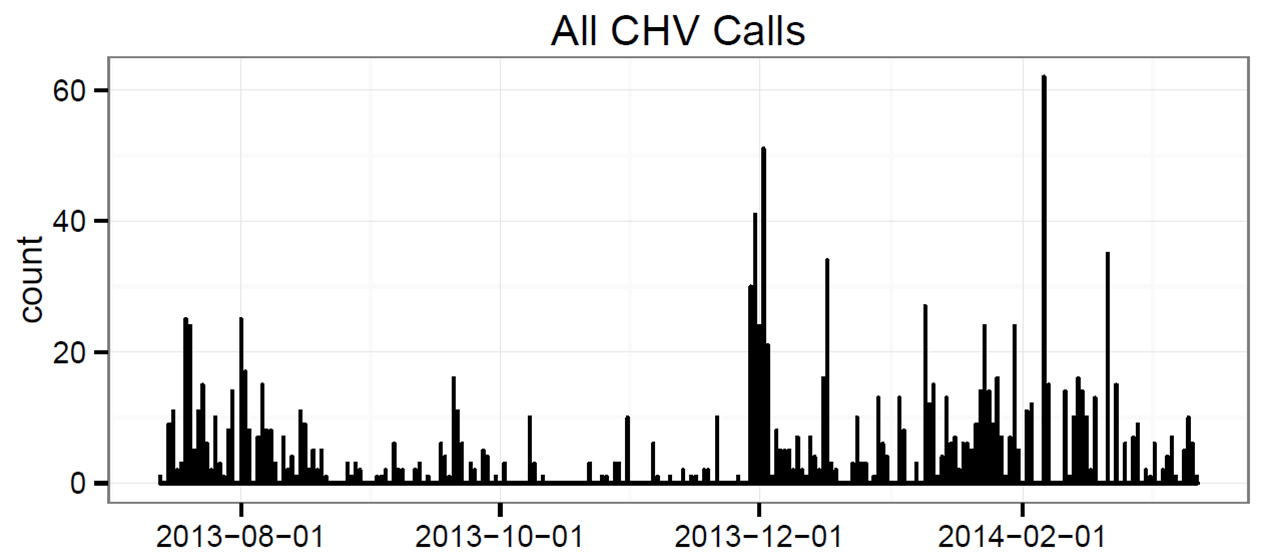
\includegraphics[width=4.5in]{all-calls}
	\end{center}
	\caption[All CHV Calls]{A total of 1,312 calls were registered to Baby Monitor from phone numbers linked to CHVs working in the study area. Call volume was generally increased over the final four months of the study compared with the first four months of the study.}
	\label{fig:allCHVcalls}
\end{figure}

\paragraph{However, not all 1,312 calls from CHVs were found to be for the purposes of engaging with the system. In only 401 calls (30.6\% of all calls)  did the CHVs press '4', the designated key for reporting an emergency, or '6', the designated key for reporting either a home visit or delivery. Call volume from these valid calls can be seen in Fig~\ref{fig:validCHVcalls}. Call volume fluctuated in a similar manner gradually decreasing over the first four months and increasing over the final four months.}

%\paragraph{In these calls, CHVs reported 95 total home visits, 22 deliveries, and XX emergencies over the eight month observation period. The research team also noted that some CHVs may have reported deliveries through the prompt intended for use by patients or families. When including these calls, CHVs reported 71 total deliveries. The remaining X calls from CHVs were unable to be completed. As part of the parallel Baby Monitor screening study, which involved data collection from 175 enrolled pregnant women, 72 reported that they delivered during the eight month study period. Thus, CHVs using the patient management system were able to account for 71 of 72 births (98.6\%) in the study catchment area, with only one birth being unaccounted for by the CHVs.}

\paragraph{In these calls, CHVs reported 95 total home visits and 22 deliveries over the eight month observation period. The research team also noted that some CHVs may have reported deliveries through the prompt intended for use by patients or families. When including these calls, CHVs reported 71 total deliveries. The remaining calls from CHVs were unable to be completed. As part of the parallel Baby Monitor screening study, which involved data collection from 175 enrolled pregnant women, 72 reported that they delivered during the eight month study period. Thus, CHVs using the patient management system were able to account for 71 of 72 births (98.6\%) in the study catchment area, with only one birth being unaccounted for by the CHVs.}

\begin{figure}[h]
	\begin{center}
	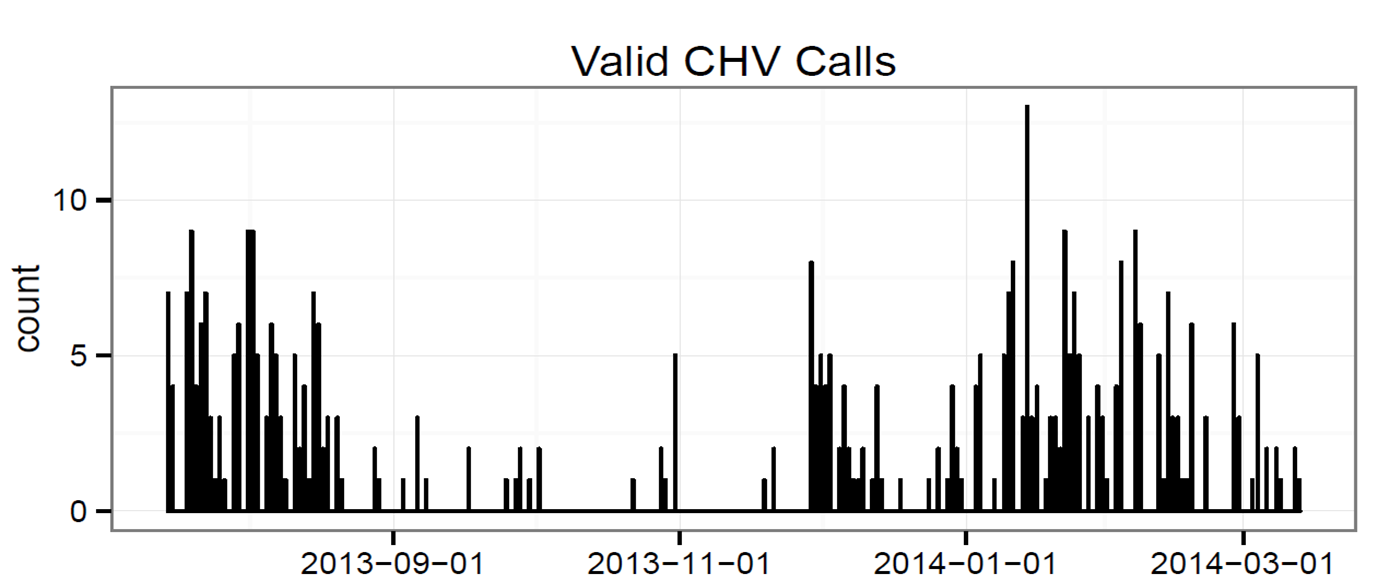
\includegraphics[width=4.5in]{valid-calls}
	\end{center}
	\caption[Valid CHV Calls]{A total of 401 calls were registered to the system from CHVs with the intent of reporting a home visit, delivery, or emergency. Call volume for these valid calls fluctuated in a similar manner as the total number of calls, with generally increased volume over the final four months of the study period.}
	\label{fig:validCHVcalls}
\end{figure}

\subsubsection{Usability Testing Results}
\paragraph{Results of the usability testing survey were generally positive. Response rate was very high among participating CHVs; 53 out of 55 (96\%) of users responded to the survey. Results corresponding to each item of the usability evaluation scale can be found in Fig ~\ref{fig:barchart}.} 

\begin{figure}[h]
	\begin{center}
	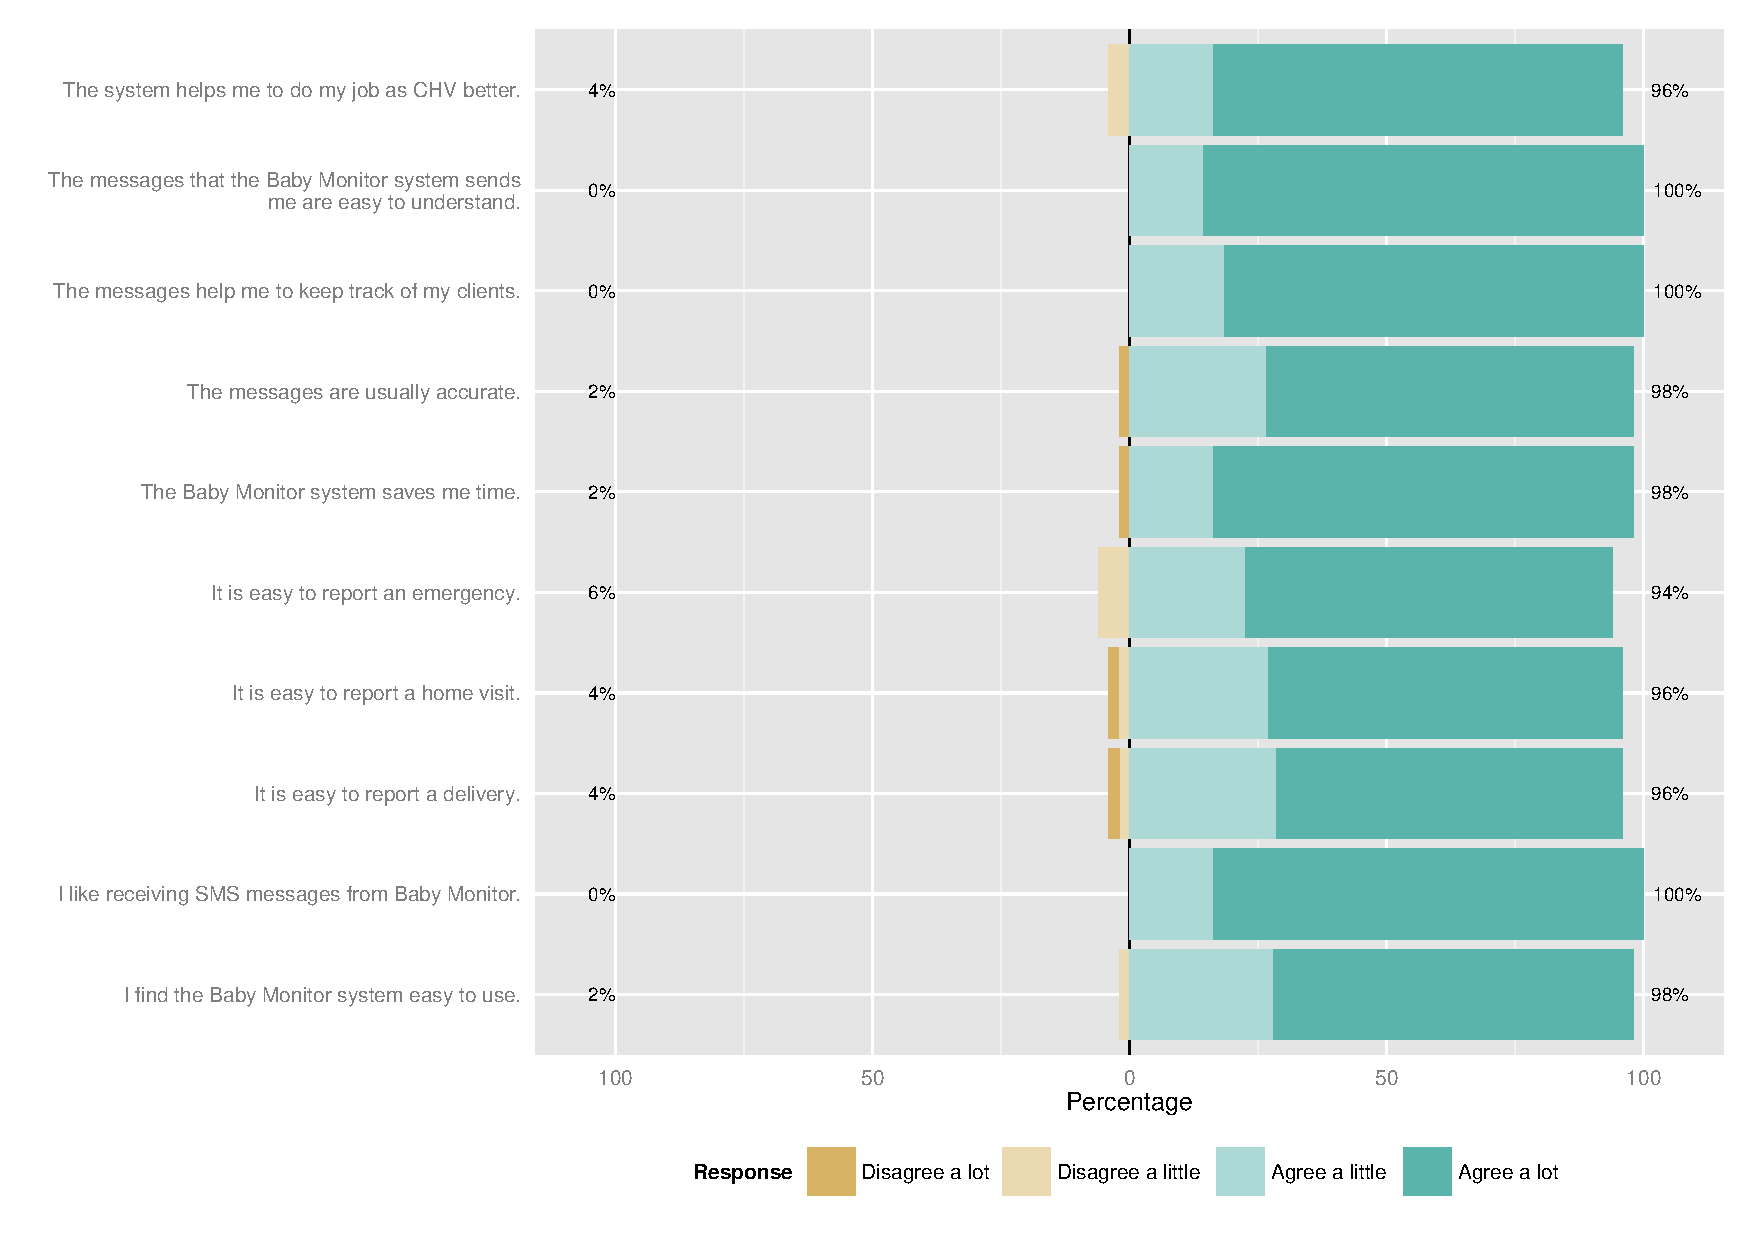
\includegraphics[width=6in]{usability-bar-316}
	\end{center}
	\caption[Usability survey results]{CHVs generally found the service to be usable. The SMS messages sent by the system were among the highest rated features of the system. Overall, 94\% of respondents believed that the system helped them do their jobs as CHVs better than before.}
	\label{fig:barchart}
\end{figure}

\paragraph{Perceived ease of use of the system was relatively high. 70\% of respondents strongly agreed that the overall system was easy to use, while 28\% moderately agreed and 2\%  moderately disagreed.Perceived usefulness of the system was also very high. 100\% of respondents agreed that they liked receiving messages from the system. 100\% of respondents also agreed that the messages help them keep track of their clients, with 81.6\% strongly agreeing with this notion. 98\% of respondents agreed that the system saved them time, 81.6\% of which strongly agreed.}

\paragraph{Respondents indicated that interacting with the system was relatively simple.  Approximately 96\% of respondents agreed that it was easy to report a home visit, while 2\% moderately disagreed and 2\% strongly disagreed. Similar trends emerged for respondents' evaluation of the delivery reporting system. 96\% of respondents  agreed that delivery reporting was easy, while 2.0\% moderately disagreed and strongly disagreed. Ease of use for emergency reporting was slightly lower. 94\% of respondents agreed that emergency reporting was easy, while 6\% disagreed. The text messaging elements of user interaction were rated very highly among respondents. 100\% of respondents agreed that the messages were easy to understand, and 100\% also agreed that the messages were usually accurate.}

\paragraph{Finally, quality of work life with the system was rated to be relatively high. 94\% of all respondents (76\% strongly agreeing and 18\% moderately agreeing) believed that the system helped them do their jobs as CHVs better than before.}




